\section{Autonomous control}
\begin{frame}{System levels}
    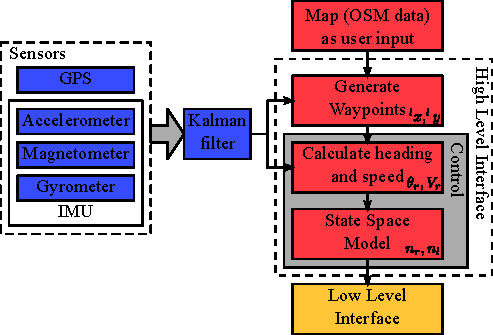
\includegraphics[width = \textwidth]{control/img/vessel-block-overview}
\end{frame}

\begin{frame}{HLI features}
		\begin{itemize}
			\item Model-based development that allows multiple Ship instances
			\centering
			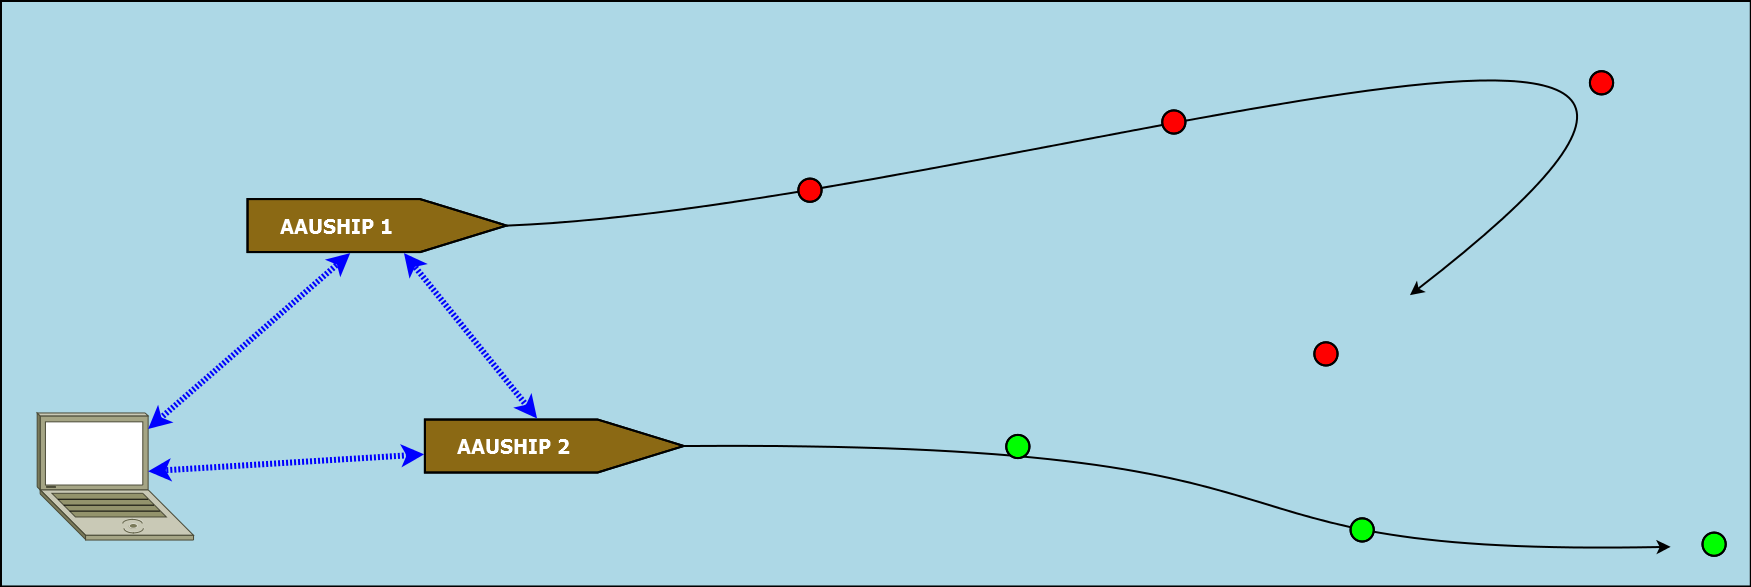
\includegraphics[trim = 5mm 5mm 5mm 5mm, clip, width = 0.8\textwidth]{control/img/actor-model}
			\item Seamlessly integrated custom Simulation environment
			\centering
			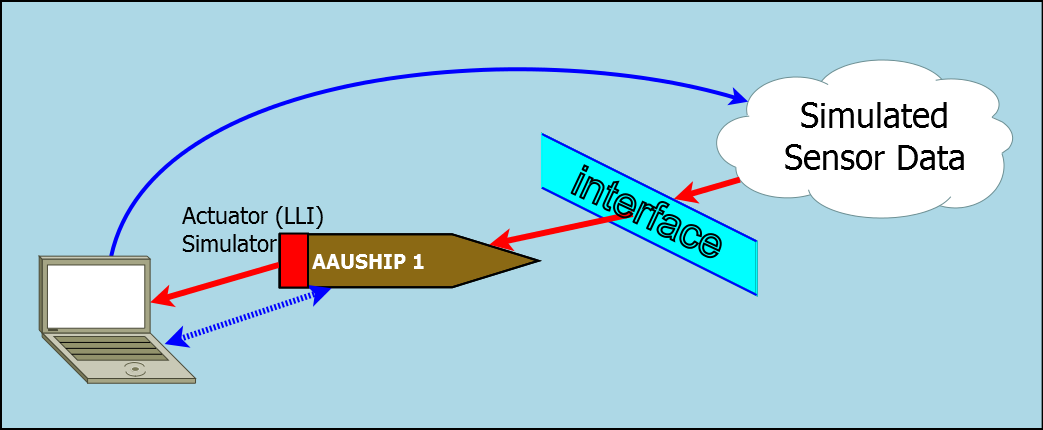
\includegraphics[trim = 5mm 5mm 5mm 5mm, clip, width = 0.8\textwidth]{control/img/simmodel}
		\end{itemize}
\end{frame}
%%%%%%%%%%%%%%%%

\subsection{Path Planning}
\begin{frame}{Waypoints and Sub-Waypoints}
    \begin{block}{Waypoints}
		\begin{itemize}
			\item Key points of interest, defining the \textbf{approximate path}
			\item Coastal information \textbf{known} $\rightarrow$ \textbf{automatic} WP generation
			\item Coastal information \textbf{unknown} $\rightarrow$ \textbf{manual} WP placement
		\end{itemize}
    \end{block}
    \begin{block}{Sub-Waypoints}
		\begin{itemize}
			\item Specific locations that the ship must approach
			\item Placed in the $\lambda_{max}$ surrounding of the \textbf{approximate path}
			\item The ship approaches each \textbf{SWP} at least to $\varepsilon$ \textbf{follow distance}
			\item Each Waypoint is approached to \textbf{at least} $\lambda + \varepsilon$ distance
		\end{itemize}
	\end{block}
\end{frame}
%%%%%%%%%%%%%%%%

\begin{frame}{Local path planning}
		\begin{itemize}
			\item Key points are determined to define an \textbf{Euler Spiral} $\rightarrow$ \textbf{Circular} $\rightarrow$ \textbf{Euler Spiral} path
			\item The centrifugal force affecting the body of the ship changes continuously and linearly
			\item The resulting sideways-movement is kept to a minimum and the control signal is better conditioned
		\end{itemize}
			\begin{tabular}{l l}
			\hspace{-3.1mm}
				\begin{minipage}{0.6\textwidth}
					\begin{itemize}
						\vspace{-2.5mm}
						\item The path is populated with Sub-Waypoints and transformed to the proper position on the map 
						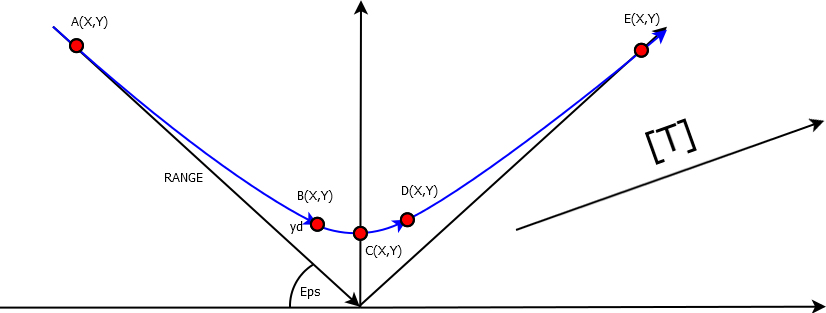
\includegraphics[width = \textwidth]{control/img/positioning1}
					\end{itemize}
				\end{minipage}
			&
				\begin{minipage}{0.3\textwidth}
					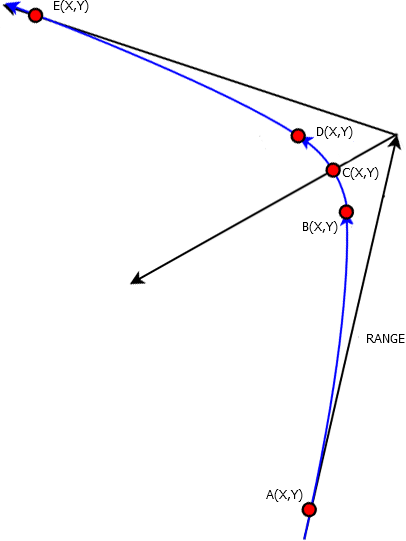
\includegraphics[width = \textwidth]{control/img/positioning2}
				\end{minipage}
			\end{tabular}
			
		
\end{frame}

%%%%%%%%%%%%%%%%
\subsection{Ship Model}
\begin{frame}{Modeling}{System Dynamics}
The Dynamics of the system are given by the drag the ship experiences when moving through the water. The drag is given as:
\begin{align}
F_\text{Drag}(\dot{x},\dot{y}) = \frac{1}{2} \cdot \rho \cdot C_\text{D} \cdot \dot{x}^2 \cdot A 
\end{align}
The formula changes when the ship is turning, as the drag then is converted into a torque - which is defined as:
\begin{align}
\tau_\text{Drag}(\omega) = \frac{1}{2} \cdot \rho \cdot C_\text{D} \cdot (d \cdot (r_f^4 + r_b^4)) \cdot \omega^2
\end{align}
The above can be put an matrix form as:
\begin{align}
\mathbf{A}\mathbf{x} = \begin{bmatrix}
-\beta_X & 0 & 0\\
0 & -\beta_Y & 0\\
0 & 0 & -\beta_\omega
\end{bmatrix}\begin{bmatrix}
\dot{x}\\
\dot{y}\\
\dot{\theta}
\end{bmatrix}
\end{align}
\end{frame}

%%%%%%%%%%%%%%%%
\begin{frame}{Modeling}{System Dynamics}
As the motion in the $y$-direction is uncontrollable, and the thing to be controlled is the velocity and the angle, the combined system becomes:
\begin{align}
\dot{\mathbf{x}} &= \mathbf{A}\mathbf{x} + \mathbf{B}\mathbf{u}\\
\begin{bmatrix}
\ddot{x}\\
\dot{\theta}\\
\dot{\omega}
\end{bmatrix} &= \begin{bmatrix}
\frac{-\beta_x}{m} & 0 & 0\\
0 & 0 & 1\\
0 & 0 & \frac{-\beta_\omega}{I}
\end{bmatrix}\begin{bmatrix}
\dot{x}\\
\theta\\
\omega
\end{bmatrix} + \begin{bmatrix}
\frac{1}{m} & 0\\
0 & 0\\
0 & \frac{1}{I}
\end{bmatrix}\begin{bmatrix}
F_\text{total}\\
\tau
\end{bmatrix}
\end{align}
And the output of the system $\mathbf{y}$ becomes:
\begin{align}
\mathbf{y} &= \mathbf{C}\mathbf{x} + D\mathbf{u}\\
\begin{bmatrix}
\dot{x}\\
\theta\\
\end{bmatrix} &= \begin{bmatrix}
 1 & 0 & 0\\
 0 & 1 & 0
\end{bmatrix}\begin{bmatrix}
\dot{x}\\
\theta\\
\omega
\end{bmatrix} + \mathbf{0}\begin{bmatrix}
F_\text{total}\\
\tau
\end{bmatrix}
\end{align}
\end{frame}

\subsection{Control system}
\begin{frame}{Navigation}
    \begin{block}{Navigation}
		\begin{tabular}{l l}
		\begin{minipage}{0.45\textwidth}
		\begin{itemize}
			\item The ship is always heading for the next Sub-Waypoint, outside of the $\varepsilon$ \textbf{follow distance}
			\item The output of the Navigator is the \textbf{reference heading} $\Theta_r$
			\item The image shows a simulation of the navigation and control based on noisy inputs
		\end{itemize}
		\end{minipage}
		&
		\begin{minipage}{0.50\textwidth}
		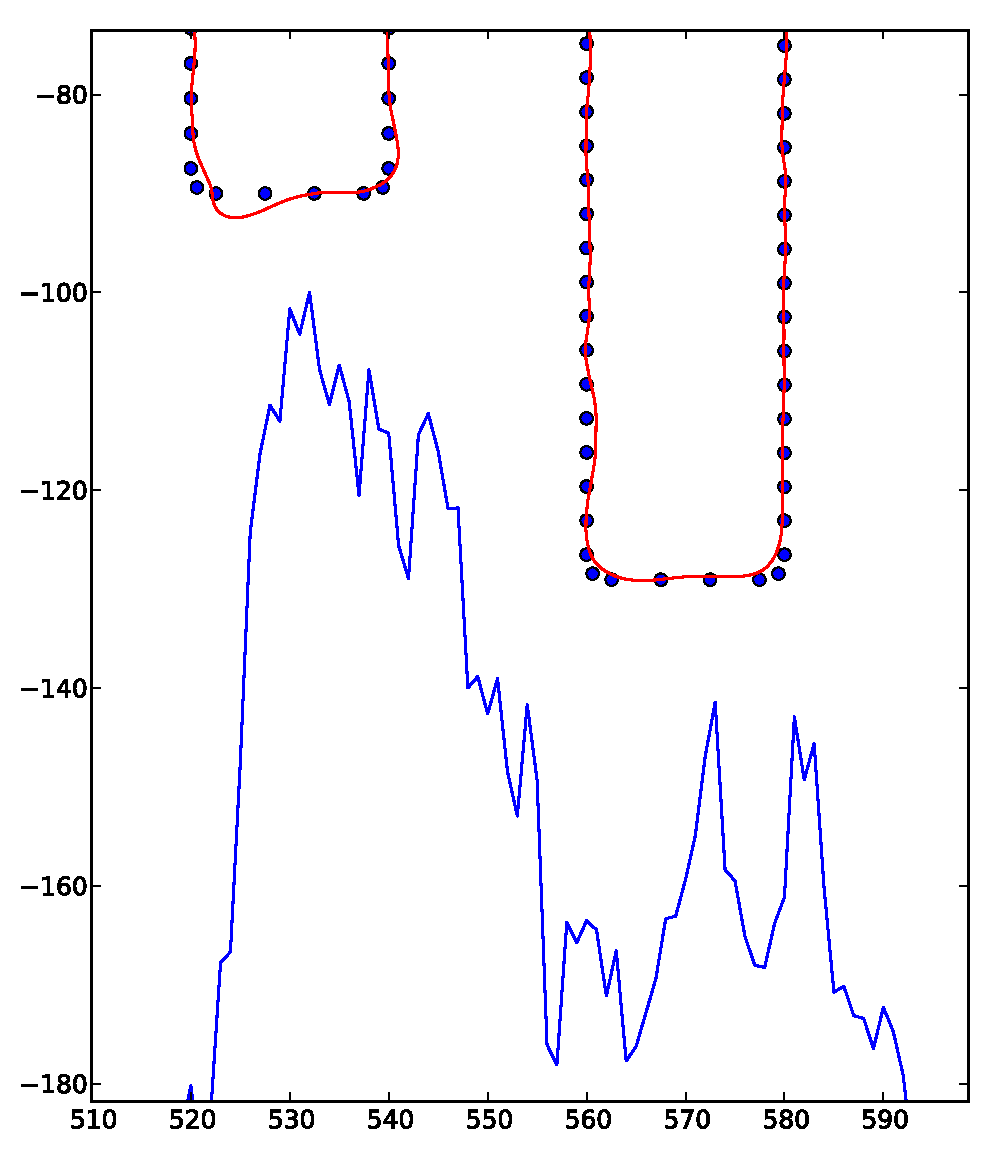
\includegraphics[width=\textwidth,keepaspectratio]{control/img/navi}
		\end{minipage}
		\end{tabular}
    \end{block}
\end{frame}

\begin{frame}{Engine controller}
    \begin{block}{Navigation}
		\begin{itemize}
			\item The engine controller is based on the linearized State-Space model
			\item Overview of the control system:
		\end{itemize}
		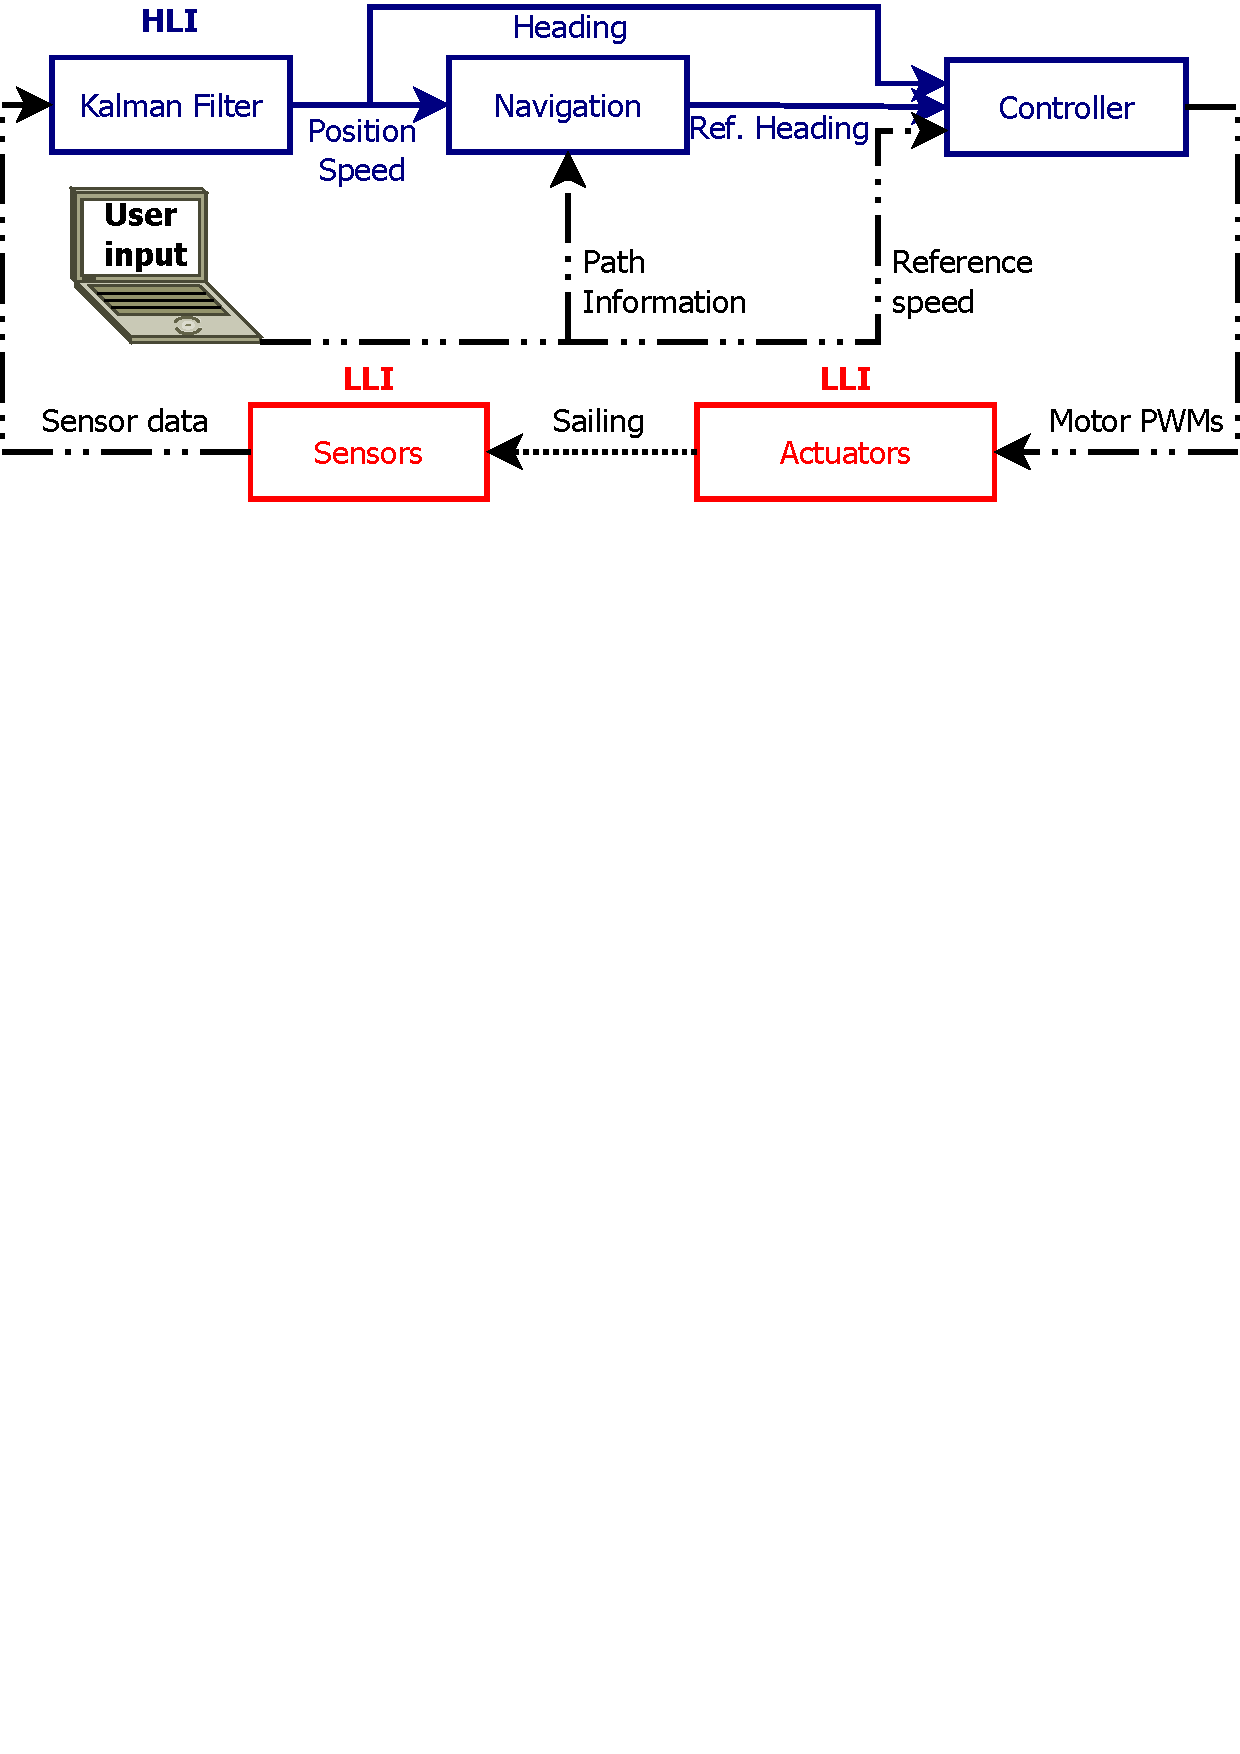
\includegraphics[trim = 0mm 21cm 0mm 0mm, clip, width=\textwidth]{control/img/controlloop}
    \end{block}
\end{frame}
%%%%%%%%%%%%%%%%